\documentclass[a4paper]{article}

\usepackage[margin=5mm]{geometry}
\usepackage{tikz,pgfplots}
\usetikzlibrary{matrix,arrows,calc,shadows,positioning,patterns,backgrounds}

\usepgfplotslibrary{external} % creates a tight self-contained pdf figure for each tikzpicture
\tikzexternalize % comment out to debug if latex errors: generates the external pdf
\tikzset{external/force remake} % otherwise will use external pdf
%\tikzsetexternalprefix{fig/} % output the pdf to an existing directory (needs to exist)

\tikzset{png export/.style={
	external/system call={
		pdflatex \tikzexternalcheckshellescape
			-halt-on-error -interaction=batchmode -jobname "\image" "\texsource";
		sips -s dpiWidth 600 -s dpiHeight 600 -s format png --out "\image.png" "\image.pdf" % sips: scriptable image processing system.
	}}}

\pgfplotsset{compat=1.12}

\tikzset{png export}

\begin{document}
\thispagestyle{empty}

\tikzsetnextfilename{myfigure}

%\scalebox{2}{
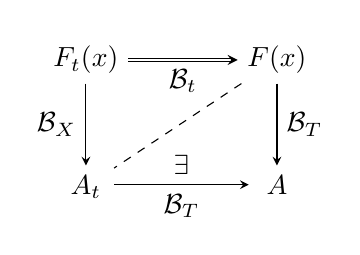
\begin{tikzpicture}
%  \begin{pgflowlevelscope}{\pgftransformscale{5}}
	\matrix (m) [matrix of math nodes,row sep=3em,column sep=4em,minimum width=2em]
	{
		F_t(x) \pgfmatrixnextcell F(x) \\
		A_t \pgfmatrixnextcell A \\};
	\path[-stealth]
		(m-1-1) edge node [left] {$\mathcal{B}_X$} (m-2-1)
						edge [double] node [below] {$\mathcal{B}_t$} (m-1-2)
		(m-2-1.east|-m-2-2) edge node [below] {$\mathcal{B}_T$}
						node [above] {$\exists$} (m-2-2)
		(m-1-2) edge node [right] {$\mathcal{B}_T$} (m-2-2)
						edge [dashed,-] (m-2-1);
%	\end{pgflowlevelscope}
\end{tikzpicture}
%}

\end{document}